\documentclass[12pt, a4paper, oneside]{ctexart}
\usepackage{amsmath, amsthm, amssymb, bm, color, framed, graphicx, hyperref, mathrsfs}
\usepackage{enumerate}
\usepackage{epstopdf}
\usepackage{float}
\usepackage{framed}
\usepackage[ruled,vlined]{algorithm2e}
\title{\textbf{assignment10}}
\author{Xiaoma}
\date{\today}
\linespread{1.5}
\definecolor{shadecolor}{RGB}{230, 245, 255}
\newcounter{problemname}
\newenvironment{problem}{\begin{shaded}\stepcounter{problemname}\par\noindent\textbf{题目\arabic{problemname}. }}{\end{shaded}\par}
\newenvironment{solution}{\par\noindent\textbf{解答. }}{\par}
\newenvironment{note}{\par\noindent\textbf{题目\arabic{problemname}的注记. }}{\par}

\begin{document}

\maketitle

\begin{problem}
\end{problem}
\begin{solution}
    \begin{enumerate}
        \item \begin{itemize}
            \item 如果存在一个最小割而边$(u,v)$不穿过它,则$c(s,t)$不变,即$| f\vert$不变,所以剩余网络中没有从$s$到
            $t$的轨。
            \item 如果存在一个最小割而边$(u,v)$穿过它,则$c(s,t)$增加一个单位,即$| f\vert$增加一个单位,所以剩余网络中
            存在从$s$到$t$的轨,进行一次$Ford-Fulkerson$循环,时间复杂度为$O(V+E)$。
        \end{itemize} 
        则该算法的时间复杂度为$O(V+E)$。
        \item \begin{itemize}
            \item 如果$(u,v)$的流量在容量减少前小于$c(u,v)$,则容量减少后,最大流不变。
            \item 如果$(u,v)$的流量在容量减少前与$c(u,v)$相等,则容量减少后,找到包含$(u,v)$的
            从$s$到$t$的路径,将该路径上所有边的流量减少一个单位,然后进行一次$Ford-Fulkerson$循环,若
            找到了新轨,则流量增加一个单位。
        \end{itemize}
        则该算法的时间复杂度为$O(V+E)$。
    \end{enumerate}
\end{solution}
\begin{problem}
    
\end{problem}
\begin{solution}
    \begin{figure}[htbp]
        \centering
        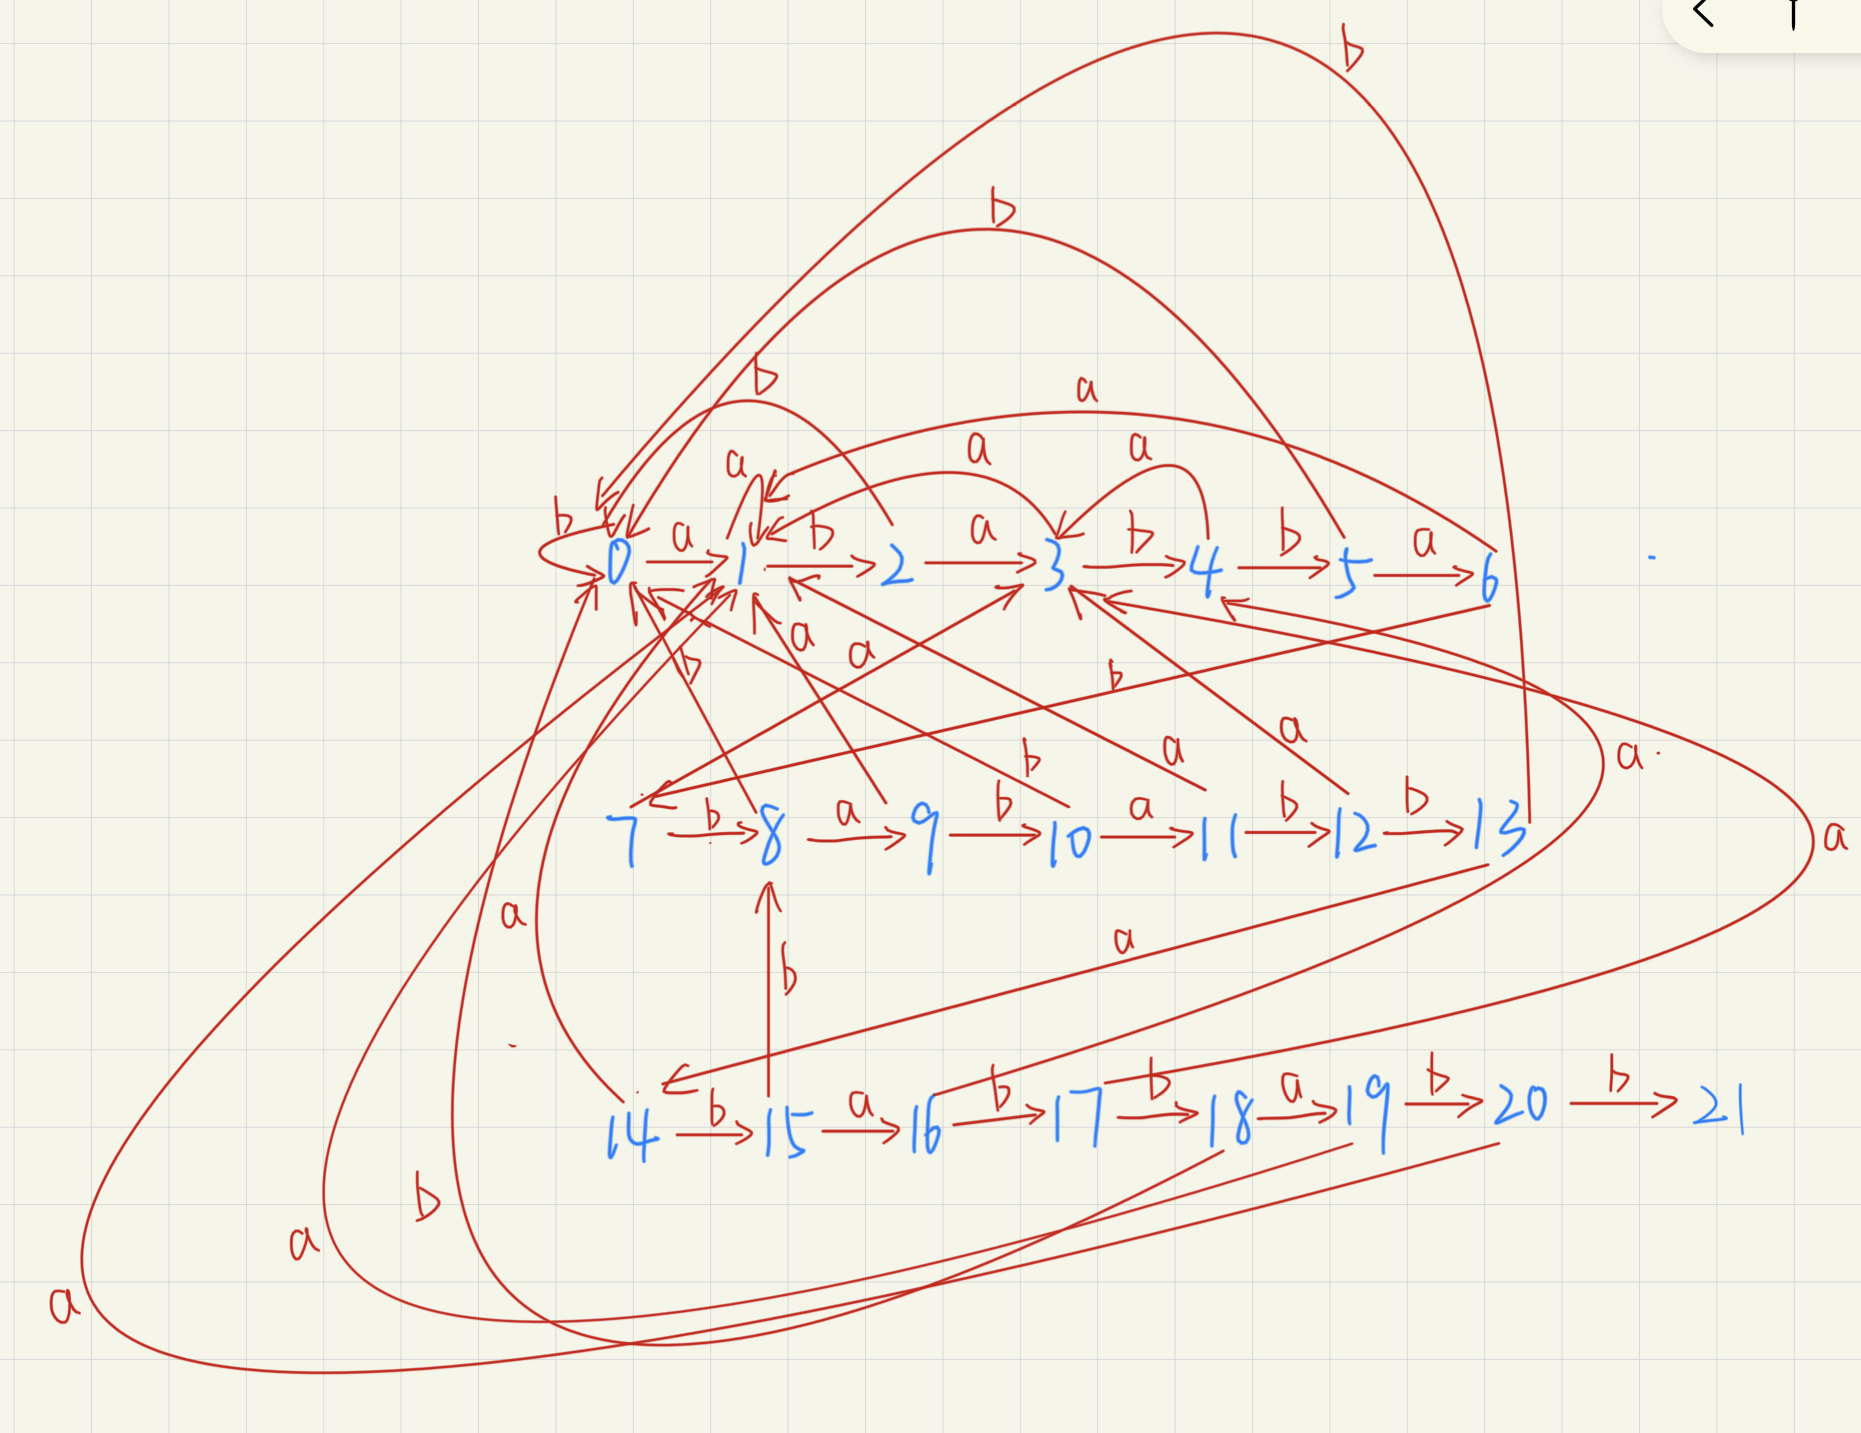
\includegraphics[scale=0.2]{1.png}
    \end{figure}
\end{solution}
\begin{problem}
    
\end{problem}
\begin{solution}
    \begin{enumerate}
        \item 设计函数$f(x,y) = (S(x) - P(y))^{2}S(x)P(y)$,翻转$P$,
        则$P(i) = B'(m-1-i)$。
        \begin{flalign*}
            F(x) = sum_{i = 0}^{m-1}(S(x - m + 1 + i) - B'(m - 1 - i))^{2}S(x - m +1+i)B'(m-1-i) \\
            =\sum_{i=0}^{m-1}S(x-m+1+i)B'(m-1-i)^{3} + \sum_{i=0}^{m-1}S(x-m+1+i)^{3}B'(m-1-i) \\- 2\sum_{i=0}^{m-1}S(x-m+1+i)^{2}B'(m-1-i)^{2}
        \end{flalign*}
        运算结果可以通过FFT得到,则时间复杂度为$O(n\log n)$。
        \item 与1同理,运算结果可以通过FFT得到,则时间复杂度为$O(n\log n)$。
    \end{enumerate}
    
\end{solution}
\end{document}